%%%%%%%%%%%%%%%%%%%%%%%%%%%%%%%%%%%%%%%%%
% Journal Article
% LaTeX Template
% Version 1.4 (15/5/16)
%
% This template has been downloaded from:
% http://www.LaTeXTemplates.com
%
% Original author:
% Frits Wenneker (http://www.howtotex.com) with extensive modifications by
% Vel (vel@LaTeXTemplates.com)
%
% License:
% CC BY-NC-SA 3.0 (http://creativecommons.org/licenses/by-nc-sa/3.0/)
%
%%%%%%%%%%%%%%%%%%%%%%%%%%%%%%%%%%%%%%%%%

%----------------------------------------------------------------------------------------
%	PACKAGES AND OTHER DOCUMENT CONFIGURATIONS
%----------------------------------------------------------------------------------------

\documentclass[twoside,twocolumn]{article}

\usepackage{blindtext} % Package to generate dummy text throughout this template 

\usepackage[sc]{mathpazo} % Use the Palatino font
\usepackage[T1]{fontenc} % Use 8-bit encoding that has 256 glyphs
\linespread{1.05} % Line spacing - Palatino needs more space between lines
\usepackage{microtype} % Slightly tweak font spacing for aesthetics

\usepackage[english]{babel} % Language hyphenation and typographical rules

\usepackage[hmarginratio=1:1,top=32mm,columnsep=20pt,left=2cm,right=2cm,top=2cm,bottom=2cm]{geometry} % Document margins
\usepackage[hang, small,labelfont=bf,up,textfont=it,up]{caption} % Custom captions under/above floats in tables or figures
\usepackage{booktabs} % Horizontal rules in tables

\usepackage{lettrine} % The lettrine is the first enlarged letter at the beginning of the text

\usepackage{enumitem} % Customized lists
\setlist[itemize]{noitemsep} % Make itemize lists more compact

\usepackage{abstract} % Allows abstract customization
\renewcommand{\abstractnamefont}{\normalfont\bfseries} % Set the "Abstract" text to bold
\renewcommand{\abstracttextfont}{\normalfont\small\itshape} % Set the abstract itself to small italic text

\usepackage{titlesec} % Allows customization of titles
\renewcommand\thesection{\Roman{section}} % Roman numerals for the sections
\renewcommand\thesubsection{\roman{subsection}} % roman numerals for subsections
\titleformat{\section}[block]{\large\scshape\centering}{\thesection.}{1em}{} % Change the look of the section titles
\titleformat{\subsection}[block]{\large}{\thesubsection.}{1em}{} % Change the look of the section titles

\usepackage{fancyhdr} % Headers and footers
\pagestyle{fancy} % All pages have headers and footers
\fancyhead{} % Blank out the default header
\fancyfoot{} % Blank out the default footer
\fancyhead[C]{Running title $\bullet$ May 2016 $\bullet$ Vol. XXI, No. 1} % Custom header text
\fancyfoot[RO,LE]{\thepage} % Custom footer text

\usepackage{titling} % Customizing the title section

\usepackage{hyperref} % For hyperlinks in the PDF

% Packages maison
\usepackage{amsmath,amssymb} % For including math equations, theorems, symbols, etc
\usepackage{mathtools}
\usepackage{bm}
\usepackage{graphicx} % Required for including images
\graphicspath{{../Figures/}} % Set the default folder for images
\usepackage{prettyref}

%----------------------------------------------------------------------------------------
%	TITLE SECTION
%----------------------------------------------------------------------------------------

\setlength{\droptitle}{-4\baselineskip} % Move the title up

\pretitle{\begin{center}\Huge\bfseries} % Article title formatting
\posttitle{\end{center}} % Article title closing formatting
\title{A database of piano and orchestral midi scores.\\Application to automatic projective orchestration} % Article title
\author{%
\textsc{John Smith}\thanks{A thank you or further information} \\[1ex] % Your name
\normalsize University of California \\ % Your institution
\normalsize \href{mailto:john@smith.com}{john@smith.com} % Your email address
%\and % Uncomment if 2 authors are required, duplicate these 4 lines if more
%\textsc{Jane Smith}\thanks{Corresponding author} \\[1ex] % Second author's name
%\normalsize University of Utah \\ % Second author's institution
%\normalsize \href{mailto:jane@smith.com}{jane@smith.com} % Second author's email address
}
\date{\today} % Leave empty to omit a date
\renewcommand{\maketitlehookd}{%
\begin{abstract}
\noindent This article introduces the \textbf{NAME} dataset, a freely-available collection of midi scores 

midi score database. It is composed by (137 OU 224 si IMSLP, mais c'est tout faux) pairs of one piano score and one corresponding orchestration. To our best knowledge, this is the first database of this kind. Thus, we also introduce a projective orchestration task, which roughly consists in learning to perform automatic orchestration of a piano score. This task can be addressed using learning methods on this database.  
\end{abstract}
}

%----------------------------------------------------------------------------------------

\begin{document}

% Print the title
\maketitle

%----------------------------------------------------------------------------------------
%	ARTICLE CONTENTS
%----------------------------------------------------------------------------------------

\section{Introduction}
% Orchestration = definition
Orchestration is the subtle art of writing musical pieces for the orchestra by combining the properties of various instruments in order to achieve a particular sonic rendering. \cite{koechli_orch,Rimsky-Korsakov:1873aa}. 
% Orchestration projective
Among the different writing techniques for orchestration, we define \textit{projective orchestration} as the technique which consists in writing first a piano score and then projecting it on an orchestra (\prettyref{fig:orch}). This technique has been long used by classic composers \textbf{(exemple ?)}.
% Dataset symbolic pour l'orchestration projective
This paper introduces what is to our best knowledge, the first symbolic dataset of projective orchestration.
% Rapide description
It contains midi scores of piano pieces, and for each of this piece, one or several corresponding orchestration(s) written by famous composers.

This database has several purposes :
\begin{itemize}
\item being the starting point for a scientific investigation of orchestration, especially for statistic-based approaches on high-level symbolic information
\item establishing a reference dataset for generative algorithms 
\item indexing works of famous composers for musicological purposes
\end{itemize}

The remainder of this paper is organized as follows. The first section introduces the structure of the database, the reason why it has been created and how informations have been gathered. In the section two, we introduce an automatic projective orchestration task. Our proposed algorithm rely on learning based methods, and uses this database. We also define an evaluation criterion that uses a part of the database. Conclusions are provided in the last section.

\section{Dataset}
\subsection{Symbolic information for orchestration}
% Teahching orchestration = exemples
Several treatise of orchestration exist \cite{koechli_orch,piston-orch,Rimsky-Korsakov:1873aa}, but they all consist in a sum of examples rather than a comprehensive theorization.
% Why ? Because it is highly complex, and we can't handle this complexity
An explanation of this observation lies in the tremendous complexity that emerges from an orchestral work. For the composer, the number of pitch and intensity ranges of each instrument is powered by the number of instruments in the orchestra, and lead to a huge combinatoric. During the performance, acoustic summation of the instruments give rise to highly non-linear effects at the signal level, which make the resulting sound almost impossible to predict. Eventually, only a little is known about the complex psycho-acoustic phenomena involved in the listening process. All those aspects play an important role in an orchestral work. Then, it seems almost impossible for a human mind to grasp in its entirety an orchestral rendering.

% Problem too complex : need for scientific investigation
Hence, we believe that a thorough scientific investigation could help disentangling the multiple factors involved in an orchestral work, and might be a precious help toward a greater understanding of the discipline.
% Scientific investigation already made ? Yes : signal et psycho-ac
If major works have already been produced in psycho-acoustic CITE and signal processing CITE, no attempts have been made to tackle orchestration from a symbolic perspective.
Here, symbolic means a scores with musical notation, as represented in \ref{fig:orch}.
% Utilité du symboliques
However, symbolic representations convey high-level information. Observing famous orchestral works from this perspective could be gratifying.
% Pourquoi pas de symbolique alors ? Complexité + pas encore les techniques adaptées
The combinatorial complexity involved by symbolic representation is directly related to the average pitch range of an instrument powered by the number of instrument. For a symphonic orchestra, we see that this complexity quickly explode. Even for a computer, an exhaustive investigation of all the possible combinations is unimaginable.
% Et maintenant on a le deep learning
But the recent advent in machine learning brought techniques that could cope with the dimensionality involved by symbolic data.
% Mais on a besoin de... DATA :)
Based on statistical tools, those techniques require a huge amount of data. Unfortunately, there is no free-access symbolic database for orchestration.
This dataset is a first attempt to fill this gap.

\begin{figure}
\centering
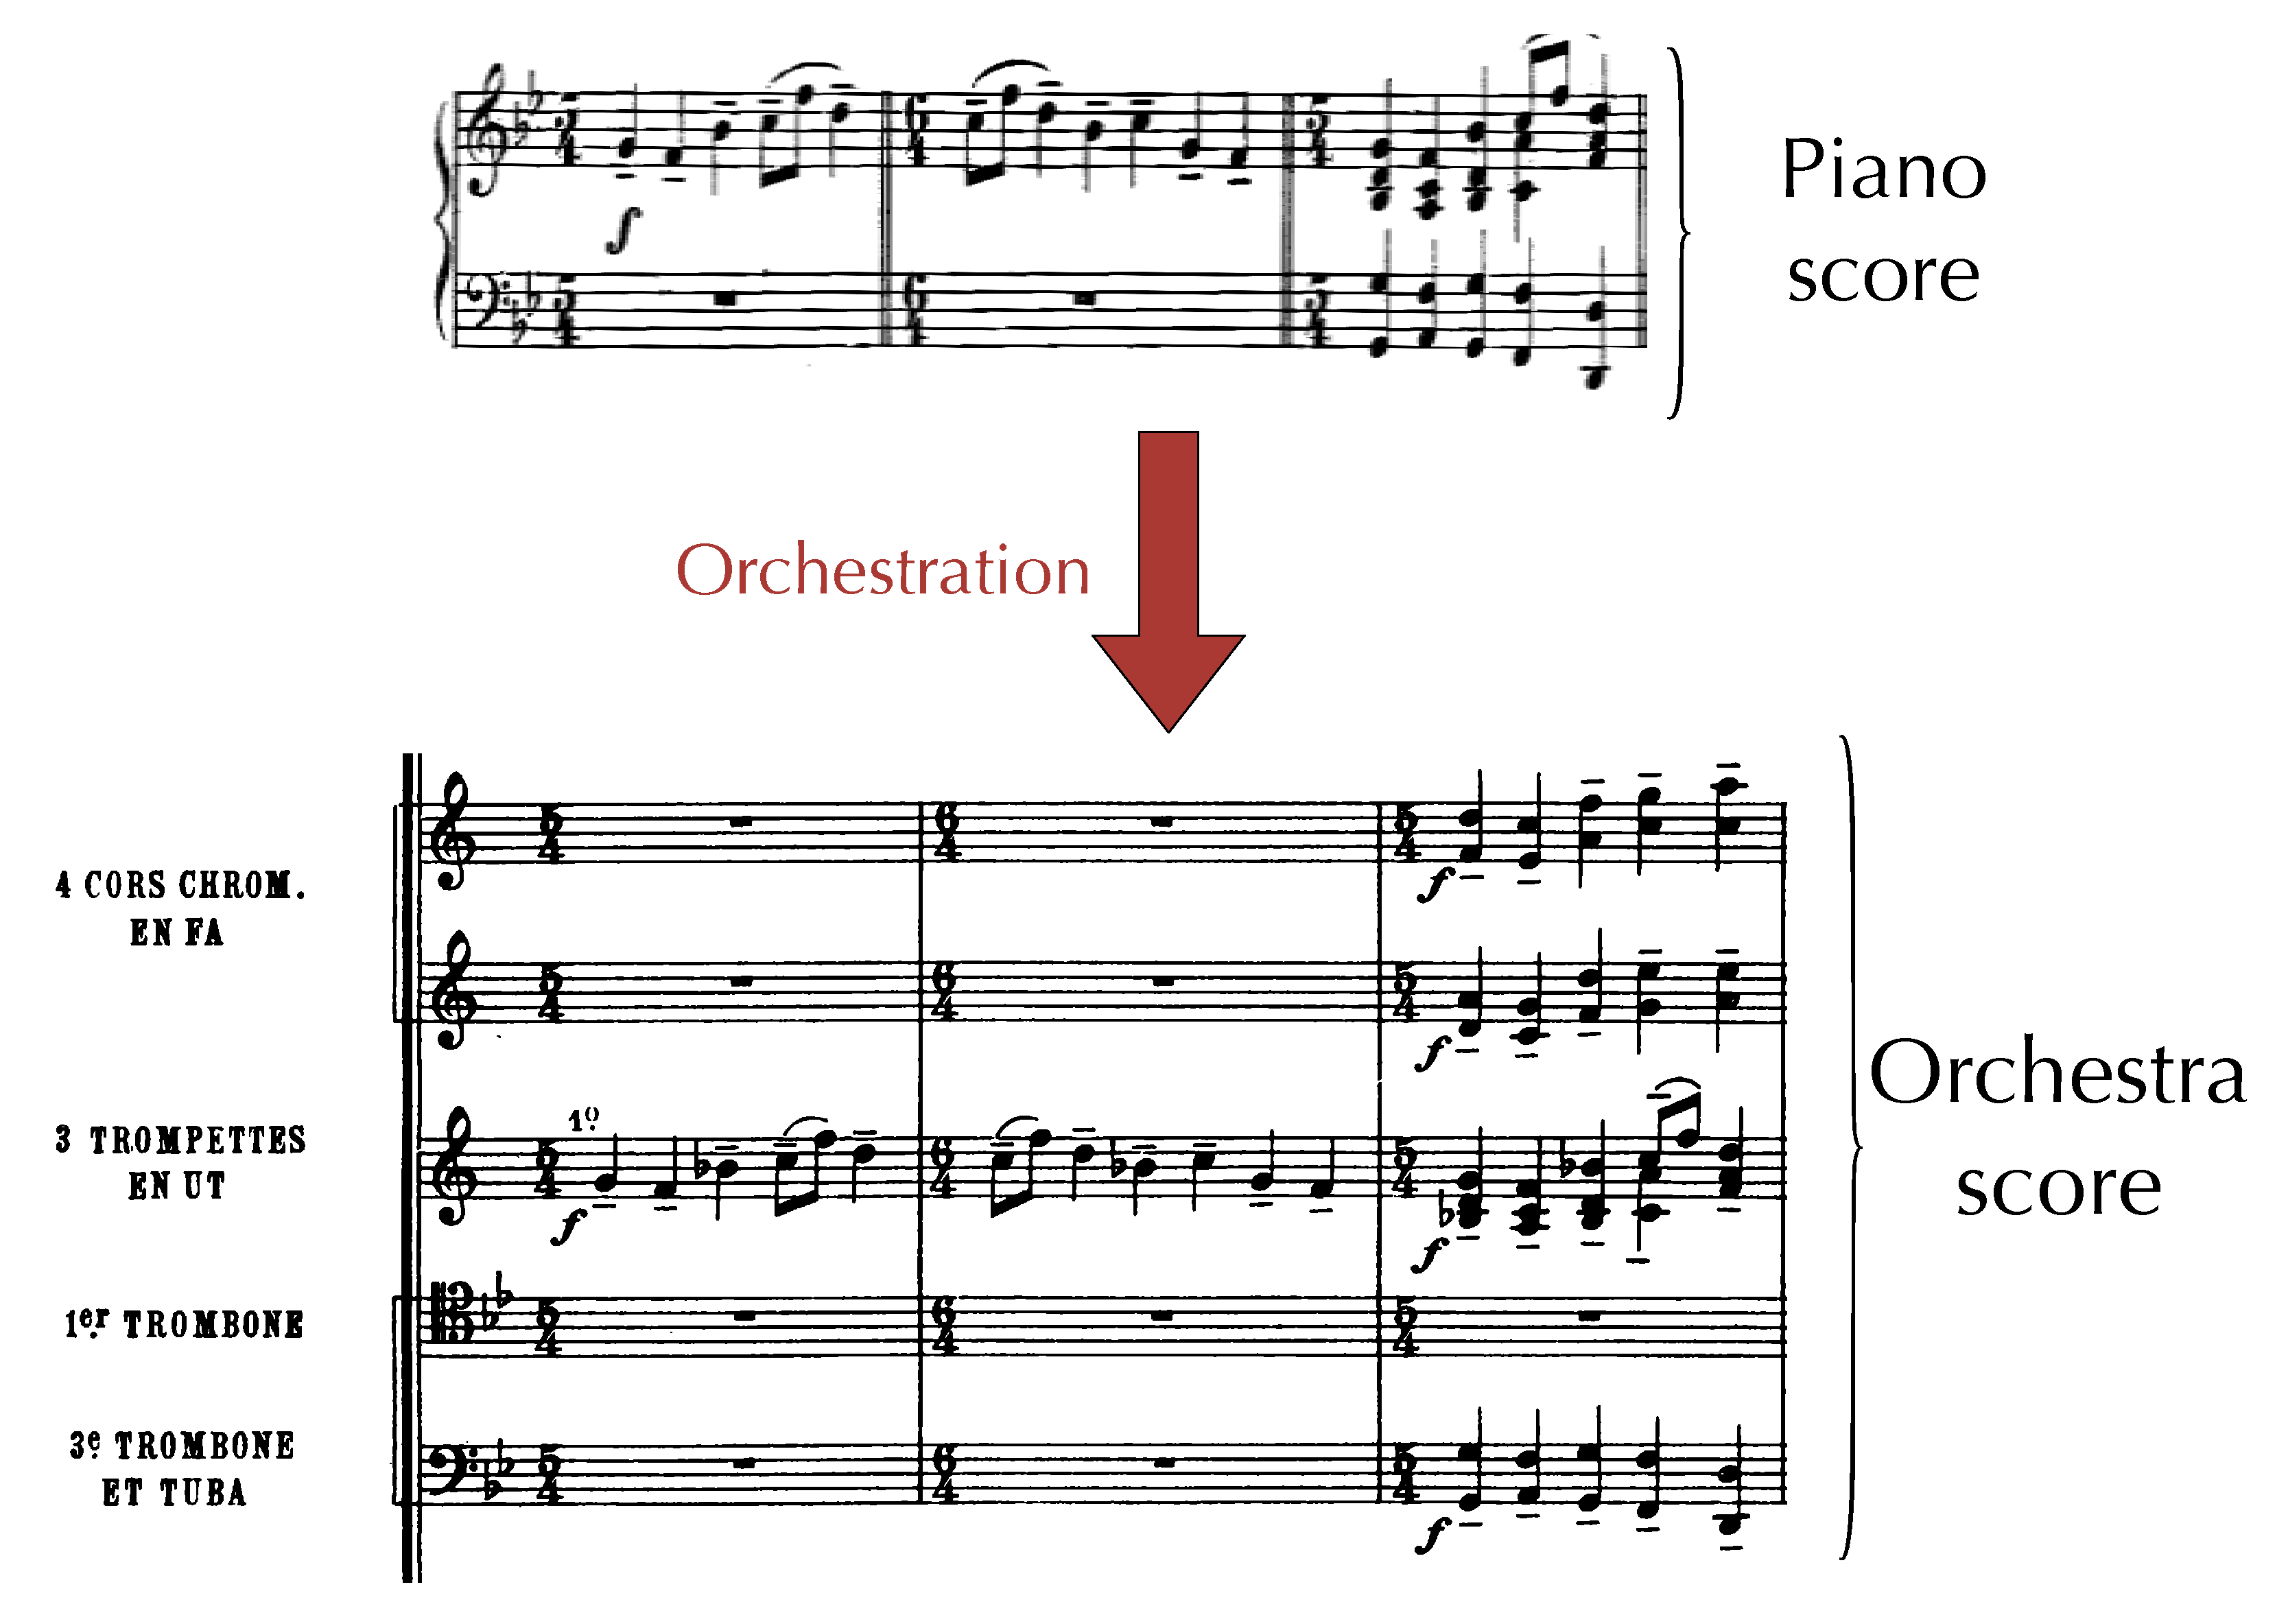
\includegraphics[scale=0.12]{orch}
\caption{\textit{Projective orchestration}. A piano score is projected on an orchestra. Even though a wide range of orchestrations exist for a given piano score, all of them will share strong relations with the original piano score. One given orchestration implicitly embeds the knowledge of the composer about timbre and orchestration.}
\label{fig:orch}
\end{figure}

\subsection{Why projective orchestration}
% Pourquoi c'est intéressant les orchestrations projectives ?
We think that projective orchestration is an extremely interesting particular case. Because orchestrating a piano piece often stem from its analysis, studying the orchestration written by a famous composer is, in a restricted way, listening to its analysis. Besides, the harmonic, rhythmic and melodic structure of a piece is already fixed in the piano score, and observing the joint information of the original piano score and an orchestrated version consists in focusing on the timbral augmentation of this primal structure. In other words, it allows to focus on how the musical discourse is highlighted by the evolution of the timbre.

\subsection{Structure of the database}
% Number of file, main aspect a+ Format midi
The \textbf{NAME} database consists in piano and orchestra scores in MIDI format.
% Organization, hierarchy
The files are grouped in folders indexed by a number. Each folder contains a pair : piano score and a possible orchestration. 
% Where does it come from
The files have been manually collected on several free-access databases found on the Internet (\textbf{CITE ??}).

% CSV instrumentation
In most orchestral midi files, one midi track is associated to one instrument. The files which were not respecting this construction have automatically been discarded. However, even for the files which respect this construction, the names of the midi tracks are often ambiguous or vague. 
Hence, a \textit{CSV} file is associated to each \textit{MIDI} file. It has the same name as the midi file. It links the name of the midi tracks to the names of an instrument, according to a nomenclature (see nomenclature.txt at the root of the folder).

% Metadata
At the root of the database folder, a \textit{metadata.csv} file can be found. It gathers, for each folder index, the relative path to the folder from the database root directory, and when available, the composer and song name for the orchestral and piano works.

% Other statistics
\textbf{General statistics about the whole database can be found in the \textit{statistics.txt} file : the number of composers, the number of instruments} \textbf{USELESS ??}.

% Manually checked
Both metadata and instrumentation csv files have been automatically generated, but manually checked. We adopted a conservative approach when sorting the files. For instance, we automatically rejected a file with the slightest ambiguity between a midi track name and an instrument and a possible instrument.

% Aligned and non-aligned versions
Two versions of the database can be downloaded. The first version contains unmodified midi files as they were originally found on the diverse websites. The second version contains midi files automatically aligned using a \textit{Needleman-Wunsch} algorithm (\textbf{CITE}). The way we used this algorithm is detailed in the next section.

% Matrices
Eventually, we offer the possibility to download a pianoroll version of the database. In this case, all the midi files of piano (respectively orchestra) work have been transformed and concatenated into one a two dimensional structure (matrix). The starting and ending time of each track is indicated in the \textit{metadata.csv} file. \textbf{Those matrices (one for the piano, one for the orchestra) can be downloaded as \textit{.mat} (Matlab) or pickle (Python) files OR JUST CSV ????}

\subsection{Construction of the database}
% Automatic search for projective orchestration match
\paragraph{Automatic search for pairs}
Freely accessible classical midi databases on the Internet contains a large number of files. Although it seems that a lot of piano and orchestra pairs can be found in those databases, it is extremely hard to link them by pair, because the metadata have not been created with this particular task in mind. Hence, we used a fuzzy string matching algorithm based on the Levenshtein distance (\cite{fuzzywuzzy}) on the names of the files to automatically detect possible piano/orchestra pairs among a database.

% Automatic alignment
\paragraph{Automatic alignment}
% Constat : toutes les partitions ne sont pas alignées
Given the diverse origins of the midi files, it often happens that a piano score and its proposed orchestration were not aligned. Indeed, one file can be shorter than the other one, because of a dilation factor or skipped parts.
% A quoi ça sert d'avoir des partitions alignées ?
Those misalignments were problematic for the learning based tasks we introduce in the next section, and in general for any processing which intends to take advantage of the joint information of the piano and orchestra score. Hence, we propose an algorithm to automatically align two symbolic scores.
% QC'est quoi aligner ? C'est aligner les séquences d'accords formées par le pianoroll
More precisely, we consider the pianoroll representations (\prettyref{fig:pianoroll}) of scores. Hence, a score can be represented as a sequence of chords. From a computational point of view, a chord is a binary vector (representing a note on or off). Note that we used a binary representations to perform alignment, but preserved the intensity in the files. Then, if we manage to define a distance between chords, the problem of aligning two scores can be casted as a classic sequence alignment problem.
% Definition pianoroll
\textbf{CHANGER LA FIGURE QUI EST CHEUM DE OUF. LA BONNE TRAINE SUR LE MAC, DANS LE DOSSIER JJCASS POSTER}
\begin{figure}[ht]
\centering
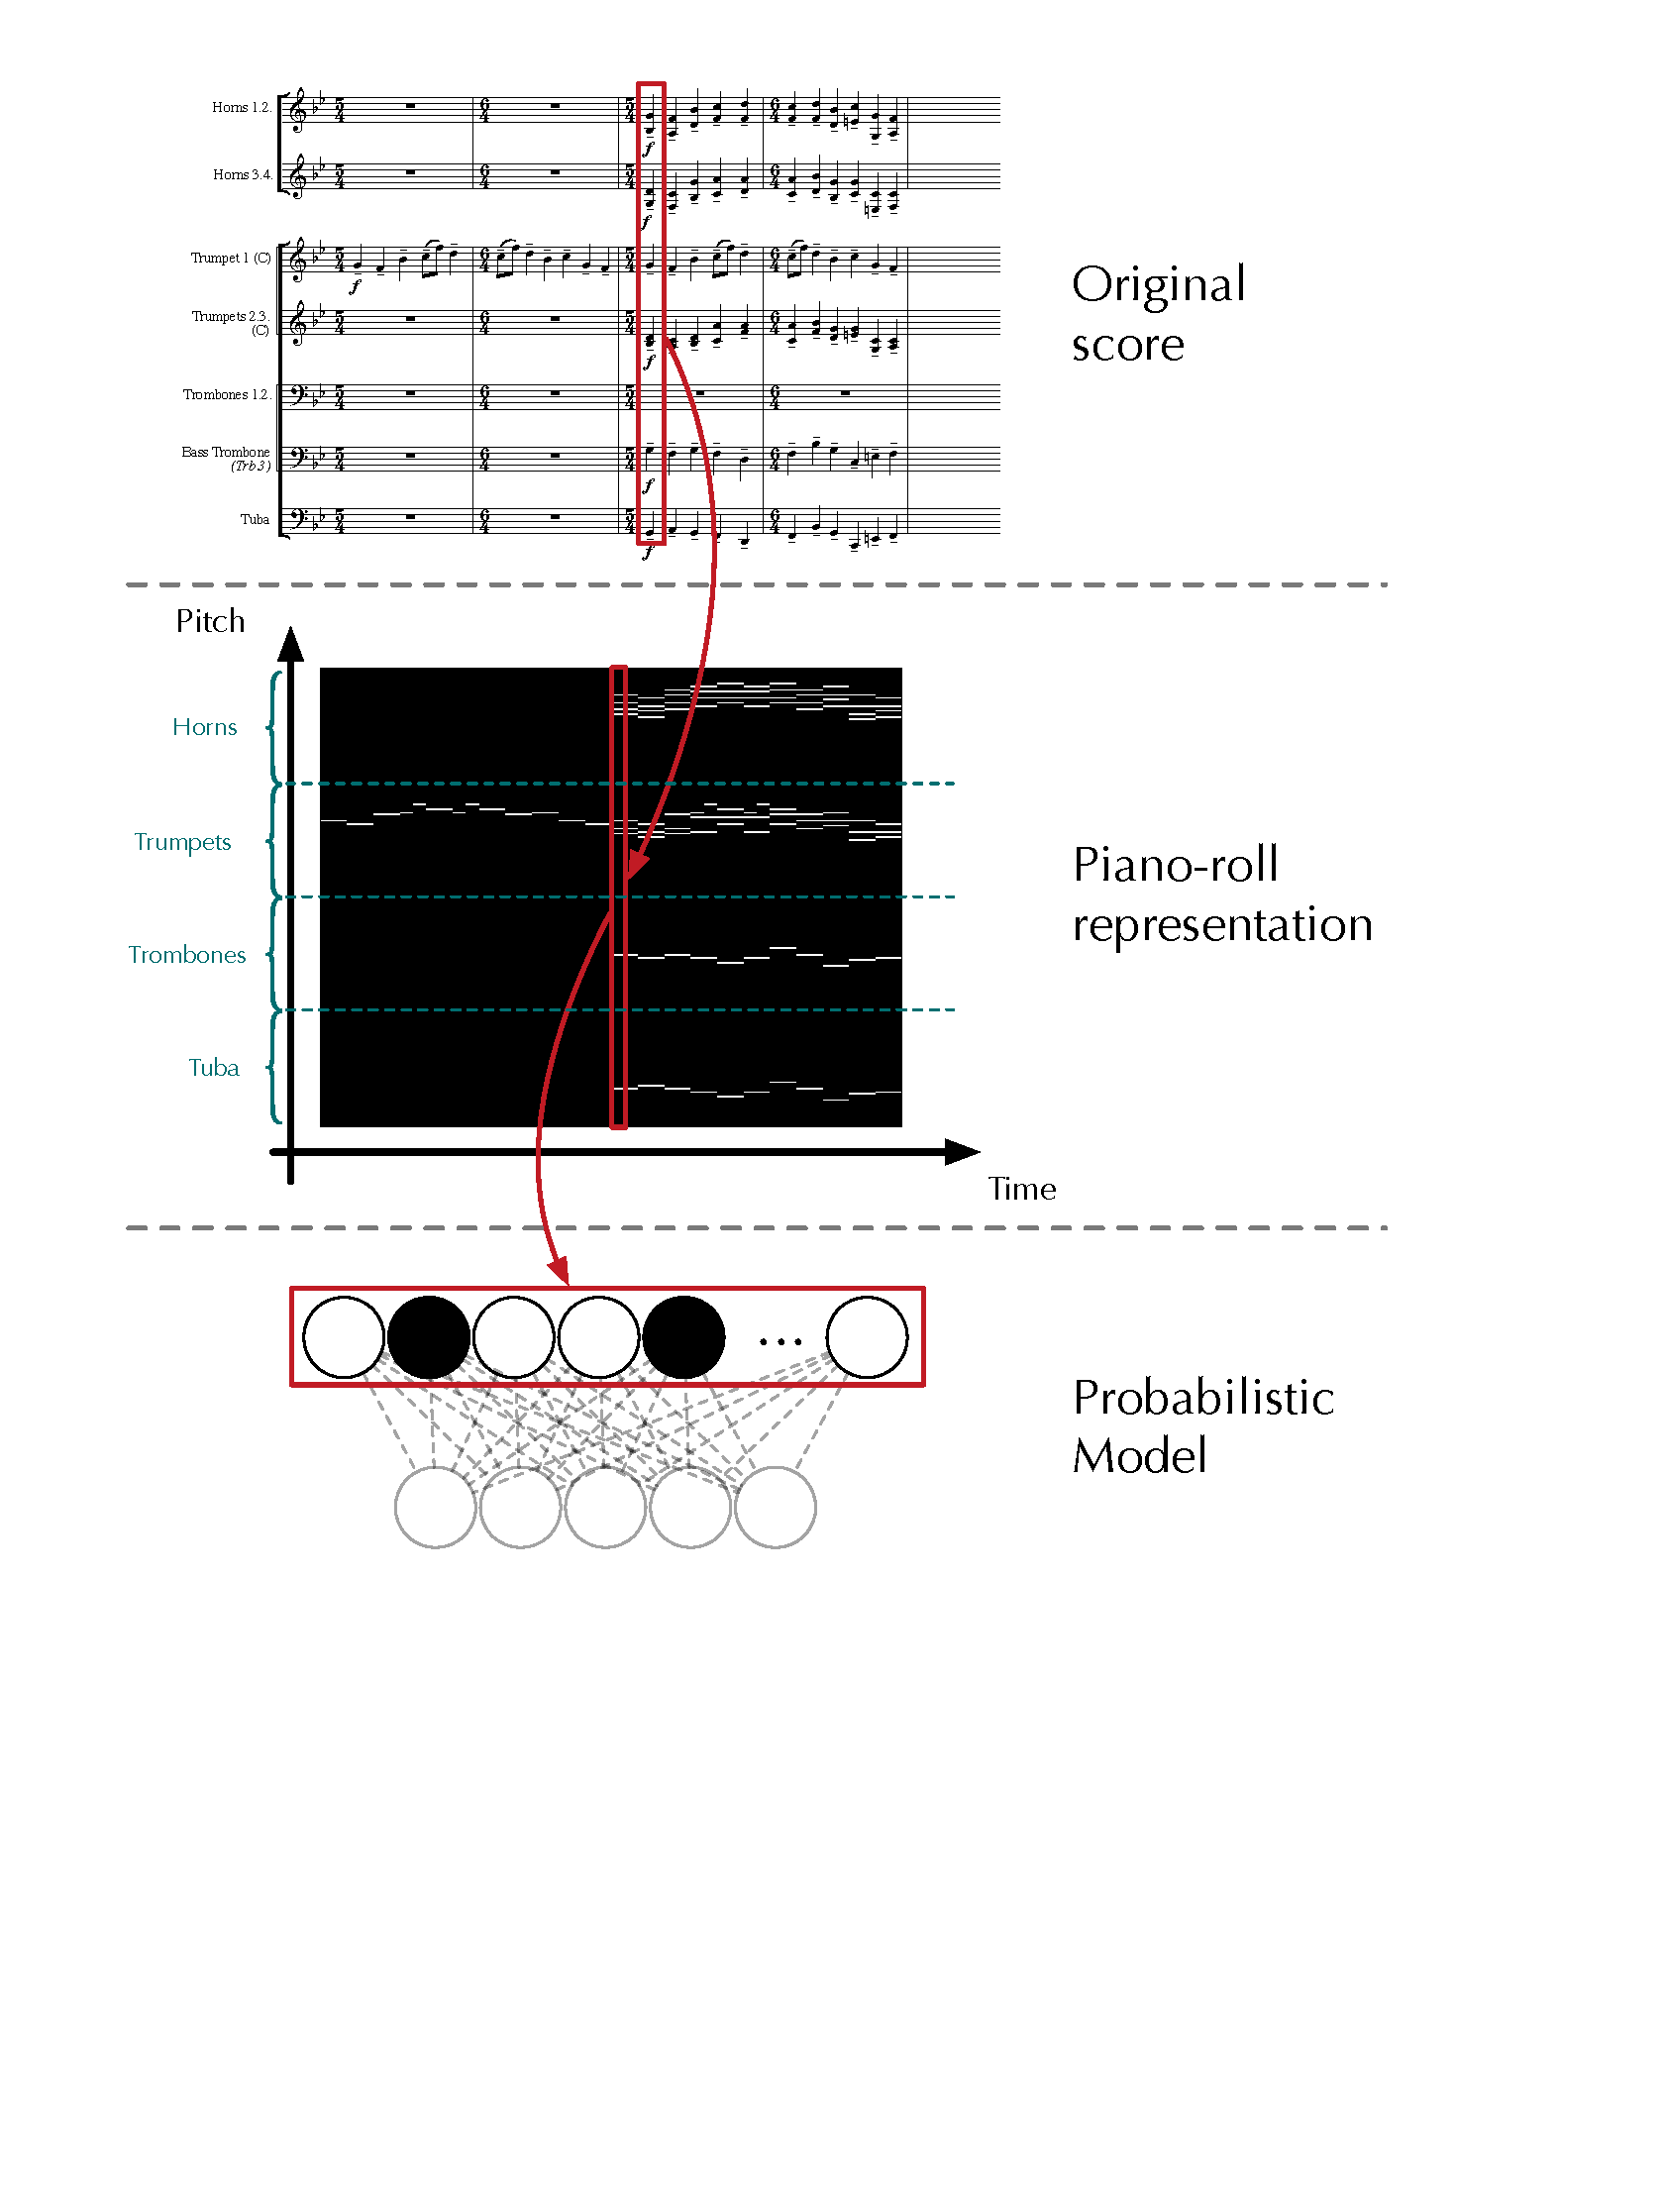
\includegraphics[scale=0.35]{data_representation}
\caption{From the score of an orchestral piece, a convenient representation for computer processing named \textit{piano-roll} is extracted. A piano-roll $pr$ is a matrix whose rows represent pitches and columns represent a time frame depending on the discretization of time. A pitch $p$ at time $t$ played with an intensity $i$ is represented by $pr(p,t) = i$, $0$ being a note off. This definition is extended to an orchestra by simply concatenating the \textit{piano-rolls} of every instruments along the pitch dimension.}
\label{fig:pianoroll}
\end{figure}

% Aligner une séquence : on sait faire = Needleman
% Description Needleman-Wunsch
Indeed, the \textit{Needleman-Wunsch}  algorithm \cite{NEEDLEMAN1970443} is a dynamic programming technique, which allows to find the optimal alignment of any two symbolic sequences, using only the introduction of gaps (\textit{i.e.} empty slots) in the sequences, but no deletion.
The only requirement of this algorithm is to be able to define a scoring system, composed by a similarity function and a gap penalty. In our case defining a similarity function boils down to building a match score between two chords.

% Similarity matrix
\paragraph{Similarity function}
We propose the following process :
\begin{itemize}
\item compute the pitch-class representation of the two chords \textbf{DETAILS}. Vectors of size 12 are obtained.
\item if one of the vector is only filled with zero, it represents a silence, and the score is set to zero.
\item else, for two pitch-class vectors A and B, we define the score as 
\begin{equation}
S =	C . \frac{\sum_{i=1}^{12} \delta(A_i , B_i)}{||A+B||_1}
\end{equation}
with
\[\delta(x) =
    \begin{cases*}
      0 & if x = 0\\
      -1 & if x = 1\\
      1 & if x = 2
    \end{cases*} 
\]
We detail the setting of the scaling factor C in the next section.
\end{itemize}

\paragraph{Tuning the algorithm}
% Gap penalty
In addition to defining a score function, the \textit{Needleman-Wunsch} algorithm has to be carefully tuned. We detail the different parameters and the value we used.
\begin{itemize}
\item the scaling factor of the similarity function ($C$) is set to 10
\item the gap open penalty defines the cost of introducing a gap in one of the two sequence. It is set to 3
\item the gap extend penalty defines the cost of extending a gap in one of the two sequence. It is to 0
\end{itemize}

% Removing the gap for BOTH scores


\textbf{SCHEMA}

\section{A case study : projective automatic orchestration}

%------------------------------------------------


%----------------------------------------------------------------------------------------
%	REFERENCE LIST
%----------------------------------------------------------------------------------------

\bibliographystyle{plain}
\bibliography{../Biblio/biblio}

%----------------------------------------------------------------------------------------

\end{document}
